\section{Lower dipolar comparison}

\begin{thm}{Theorem}
Any Alexandrov space with nonnegative curvature satisfies the tree comparison for the following two trees:

\begin{center}
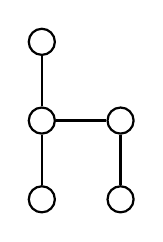
\begin{tikzpicture}[scale=1,
  thick,main node/.style={circle,draw,font=\sffamily\bfseries,minimum size=3mm}]
  \node[main node] (1) at (0,0) {};
  \node[main node] (2) at (0,1){};
  \node[main node] (3) at (0,2){};
  \node[main node] (4) at (1,0) {};
  \node[main node] (5) at (1,1) {};
  

  \path[every node/.style={font=\sffamily\small}]
   (1) edge node[above]{}(2)
   (2) edge node[above]{}(3)
   (2) edge node[above]{}(5)
   (4) edge node[above]{}(5);
\end{tikzpicture}
\hskip10mm
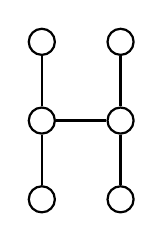
\begin{tikzpicture}[scale=1,
  thick,main node/.style={circle,draw,font=\sffamily\bfseries,minimum size=3mm}]

  \node[main node] (1) at (0,0) {};
  \node[main node] (2) at (0,1){};
  \node[main node] (3) at (0,2){};
  \node[main node] (4) at (1,0) {};
  \node[main node] (5) at (1,1) {};
  \node[main node] (6) at (1,2) {};

  \path[every node/.style={font=\sffamily\small}]
   (1) edge node[above]{}(2)
   (2) edge node[above]{}(3)
   (2) edge node[above]{}(5)
   (4) edge node[above]{}(5)
   (5) edge node[above]{}(6);
\end{tikzpicture}
\hskip10mm
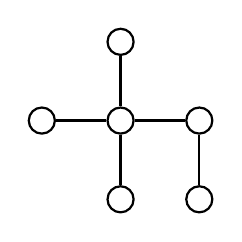
\begin{tikzpicture}[scale=1,
  thick,main node/.style={circle,draw,font=\sffamily\bfseries,minimum size=3mm}]

  \node[main node] (1) at (0,1) {};
  \node[main node] (2) at (1,0){};
  \node[main node] (3) at (1,1){};
  \node[main node] (4) at (1,2) {};
  \node[main node] (5) at (2,0) {};
  \node[main node] (6) at (2,1) {};

  \path[every node/.style={font=\sffamily\small}]
   (1) edge node[above]{}(3)
   (2) edge node[above]{}(3)
   (3) edge node[above]{}(6)
   (4) edge node[above]{}(3)
   (5) edge node[above]{}(6);
\end{tikzpicture}
\end{center}

\end{thm}

\parit{Proof.} First we will show the statement for the first tree and use this in the proofs for the second and third trees.
The latter two proofs are neraly identical.

Let us label the poles by $p_1$ and $p_2$ and the reaming 3 vertexes by $x_1,x_2,x_3$.

The required model configuration $\~p_1$, $\~p_2$, $\~x_1$, $\~x_2$, $\~x_3\in \RR^3$ will be found among the configurations where in addition the angle between $[\~p_1,\~p_2]$ and the remaining edges $[p_j,x_j]$ of the tree are the same as the corresponding angles in $A$; these type of configurations will be called \emph{pivotal}.

Up to a motion of the space, the configuration of that type is completely described by 6 angles $\alpha_{i,j}$ between the planes $\~p_1 \~p_2 \~x_i$ and $\~p_1\~p_2 \~x_j$.

Denote by $\beta_{i,j}$ the minimal angle between the planes $\~p_1 \~p_2 \~x_i$ and $p_1p_2 x_j$ such that $|\~x_i-\~x_j|_{\RR^3}\ge|\~x_i-\~x_j|_A$. 
Note that the configuration $\~p_1,\~p_2,\~x_1,\~x_2,\~x_3,\~x_4$ is valid if $\alpha_{i,j}\ge \beta_{i,j}$ for all pairs $(i,j)$.

Note that $\beta_{i,j}\le \pi$ for any pair $(i,j)$.

In other words, we need to show that if $\~p_1,\~p_2,\~x_i,\~x_j$ is a model configuration with $\alpha_{i,j}=\pi$ then 
\[|\~x_i-\~x_j|_{\RR^3}\ge |x_i-x_j|_{A}.\eqlbl{|x-x|}\]
Note that in this configuration the line segment $[\~x_i,\~x_j]$ intersects the line $\~p_1\~p_2$;
denote by $\~z$ the point of intersection.

If $\~z\in [\~p_1,\~p_2]$, consider the corresponding point $z\in [p_1,p_2]$.
In the remaining case, $\~z\notin [\~p_1,\~p_2]$, without loss of generality, we can assume that $\~z$ lies on the half line $\~p_1\~p_2$.
In this set $z$ to be the image of $p_2$ for the $(\tfrac12\cdot \dist_{p_1}^2)$-gradient flow of $p_2$ for time $t=\ln \tfrac{|\~z-\~p_1|}{|\~p_2-\~p_1|}$.
In both cases the comparsison implies 
\begin{align*}
|x_i-z|_A &\le |\~x_i-\~z|_{\RR^3},
&
|x_j-z|_A &\le |\~x_j-\~z|_{\RR^3}.
\end{align*}
From the triangle inequality, \ref{|x-x|}
follows.

Along the same lines we can show that 
\[\beta_{i,j}+\beta_{j,k}+\beta_{k,i}\le 2\cdot \pi\eqlbl{sum=<2pi}\] 
for any triple $(i,j,k)$.


Indeed, assume contrary.
Since $\beta_{i,k}\le \pi$, it follows that 
\[\beta_{i,j}+\beta_{j,k}> \pi.\eqlbl{sum>=pi}\] 
Consider a configuration $\~p_1,\~p_2,\~x_i,\~x_j,\~x_k\in\RR^3$ such that 
$\alpha_{i,j}=\beta_{i,j}$, $\alpha_{j,k}=\beta_{j,k}$ and the points $x_i$ and $x_k$ lie on the opposite sides from the plane $\~p_1\~p_2\~x_j$.
By \ref{sum>=pi}, $[\~x_i\~x_j\~x_k]$ intersects the line $\~p_1\~p_2$;
denote by $\~z$ the point of intersection.

Let us construct a point $z\in A$ which corresponds to $\~z$ the same way as above.
By construction 
\begin{align*}
|x_i-x_j|_A &= |\~x_i-\~x_j|_{\RR^3},
&
|x_j-x_k|_A &\le |\~x_j-\~x_k|_{\RR^3}.
\end{align*}
By comparison implies 
\begin{align*}
|x_i-z|_A &\le |\~x_i-\~z|_{\RR^3},
&
|x_j-z|_A &\le |\~x_j-\~z|_{\RR^3},
&
|x_k-z|_A &\le |\~x_k-\~z|_{\RR^3}.
\end{align*}
By comparison, 
\[|x_i-x_k|_A \le  |\~x_i-\~x_k|_{\RR^3};\]
hence \ref{sum=<2pi} follows.


Assume one of the triangle inequalities 
\[\beta_{i,k}\le \beta_{i,j}+\beta_{j,k}\]
does not hold.
Order the values $\{\beta_{i,j}\}$ in a nonincreasing order.
Let us construct a metric graph with 4 vertexes labeled by $\{1,2,3,4\}$
the following way choose the the largest value $\beta_{i,j}$ 
and attche an edge $(i,j)$ of length $\beta_{i,j}$,
do the same for the second largest value and so on,
starting from third step, before adding new edge we have to check that the triangle inequalities does not brake; in other words we want to 
At the end we get a metric 
\qeds